\documentclass{beamer}

\usepackage{verbatim}
\usepackage{fancyvrb}
\usepackage{amsmath}
\usepackage{mathtools}
\usepackage{booktabs}
\usepackage{amssymb}
\usepackage{graphicx}
\usepackage{calc}
\usepackage{color}
\usepackage{multicol}
\usepackage{wrapfig}
\usepackage{natbib}
\usepackage[ruled,vlined]{algorithm2e}
\usepackage{animate}
\usepackage{mathtools}
\usepackage{listings}

% two col: two columns
\newenvironment{twocol}[4]{
\begin{columns}[c]
\column{#1\textwidth}
#3
\column{#2\textwidth}
#4
\end{columns}
}

\makeatletter
\setbeamertemplate{theorem begin}
{%
\begin{\inserttheoremblockenv}
  {}{\usebeamerfont*{block title}\usebeamercolor[fg]{block title}%
  \inserttheoremname
  %\inserttheoremnumber
  \ifx \inserttheoremaddition \empty \else\ (\inserttheoremaddition)\fi
  \inserttheorempunctuation}
  \normalfont
  }
  \setbeamertemplate{theorem end}{\end{\inserttheoremblockenv}}
\makeatother

\newcommand{\E}{\mathrm{E}}
\newcommand{\Var}{\mathrm{Var}}
\newcommand{\Cov}{\mathrm{Cov}}
\newcommand{\sd}{\mathrm{sd}}
\newcommand{\se}{\mathrm{se}}
\newcommand{\Corr}{\mathrm{Corr}}
\newcommand{\rank}{\mathrm{rank}}
\newcommand{\nullspace}{\mathrm{null}}
\newcommand{\myspan}{\mathrm{span}}
\DeclareMathOperator*{\argmax}{arg\,max}
\DeclareMathOperator*{\argmin}{arg\,min}
\DeclareMathOperator*{\softmax}{softmax}

\definecolor{darkgreen}{rgb}{0,0.5,0}

\newtheorem{proposition}[theorem]{Proposition}
\newtheorem{exe}{Exercise}

\definecolor{darkgreen}{rgb}{0,0.5,0}

\title{Linear Regression with One Predictor Variable}
\author{Zhenisbek Assylbekov}
\institute{Department of Mathematics}
\date{Regression Analysis}

\AtBeginSection[]
{
  \begin{frame}<beamer>
    \tableofcontents[currentsection]
  \end{frame}
}

\begin{document}

\begin{frame}
  \titlepage
\end{frame}


\section{Model}

\begin{frame}{Introduction}
\textbf{Simple regression} is about modeling one variable  as a function of another variable
$$
y=f(x)
$$
given some data $(x_1, y_1), \ldots, (x_n, y_n)$.\\~\\

\pause Usually $f(x)$ is parameterized:
$$
y=f(x;\theta)
$$

\pause The goal is to tweak $\theta$ so that $y=f(x;\theta)$ fits the data in the best possible way.
\end{frame}

\begin{frame}
\frametitle{Poverty vs. HS graduate rate}

The \textit{scatterplot} below shows the relationship between HS graduate rate in all 50 US states and DC and the \% of residents who live below the poverty line {\small (income below \$23,050 for a family of 4 in 2012)}.

\begin{columns}
\begin{column}{0.55\textwidth}
\begin{center}
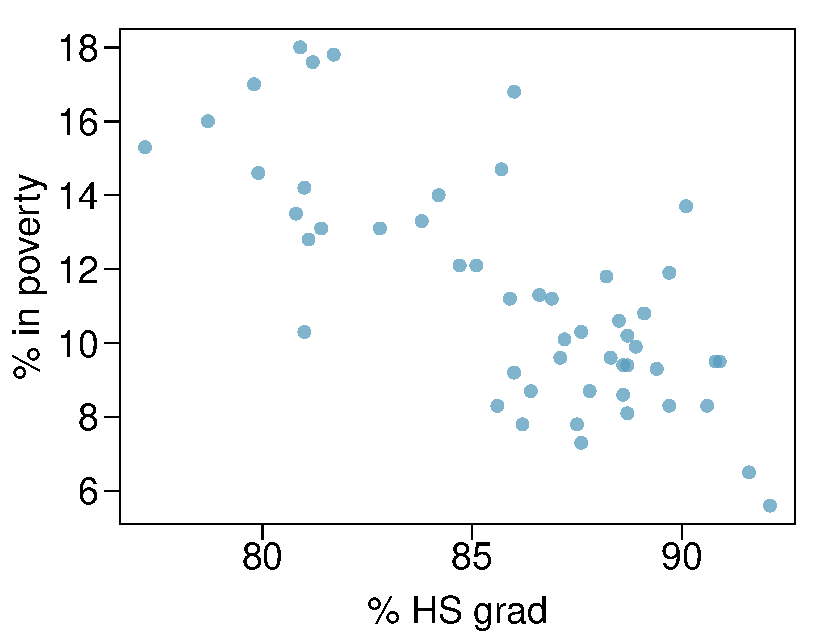
\includegraphics[width=\textwidth]{plots/poverty_hsgrad}
\end{center}
\end{column}
\begin{column}{.45\textwidth}
\pause
\textbf{Response variable} ($y$)

\pause
\% in poverty\\~\\

\pause
\textbf{Explanatory variable} ($x$)

\pause
{\% HS grad}\\~\\

\pause
\textbf{Relationship}

\pause
{linear, negative, moderately strong}
\end{column}
\end{columns}
\end{frame}


\begin{frame}{Simple linear regression model}
\begin{itemize}
    \item The simplest relationship between two variables $x$ and $y$ is linear:
    $$
    y=\beta_0+\beta_1 x
    $$
    \item<2-> To allow variability around the line we add random noise:
    $$
    Y_i=\underbrace{\beta_0+\beta_1 x_i}_{\text{deterministic}} + \epsilon_i,\quad i=1,\ldots,n,
    $$
    where
    \begin{itemize}
    \item<3-> $Y_i$ is the value of the \textbf{response variable} in the $i^\text{th}$ example,
    \item<4-> $x_i$ is the value of the \textbf{predictor variable} in the $i^\text{th}$ example.
    \end{itemize}
    \item<6->Assumptions on $\epsilon_i$'s:
    \begin{itemize}
        \item<6-> $\E[\epsilon_i]=0$
        \item<7-> $\Var[\epsilon_i]=\sigma^2$
        \item<8-> $\Cov[\epsilon_i,\epsilon_j]=0$ for $i\ne j$
    \end{itemize}
\end{itemize}
\end{frame}



\begin{frame}{Mean and variance of each $Y_i$}

Given the simple linear regression model
\begin{align*}
&Y_i=\beta_0+\beta_1 x_i+\epsilon_i,\\
&\E[\epsilon_i]=0,\quad \Var[\epsilon_i]=\sigma^2,\quad \Cov[\epsilon_i,\epsilon_j]=0\text{ for }i\ne j
\end{align*}
show that
\begin{itemize}
    \item<2-> $\E[Y_i]=\beta_0 + \beta_1 x_i$,
    \item<3-> $\Var[Y_i]=\sigma^2$,
    \item<4-> $\Cov[Y_i,Y_j]=0$.
\end{itemize}
\end{frame}


\begin{frame}{Interpretation of $\beta_0$ and $\beta_1$}
\begin{columns}
\begin{column}{.5\textwidth}
Suppose we somehow estimated $\beta_0$ and $\beta_1$ in the Poverty vs HS grads example:
$$
Y_i=64.68-0.62\cdot x_i + \epsilon_i
$$
\end{column}
\begin{column}{.5\textwidth}
\begin{figure}
    \centering
    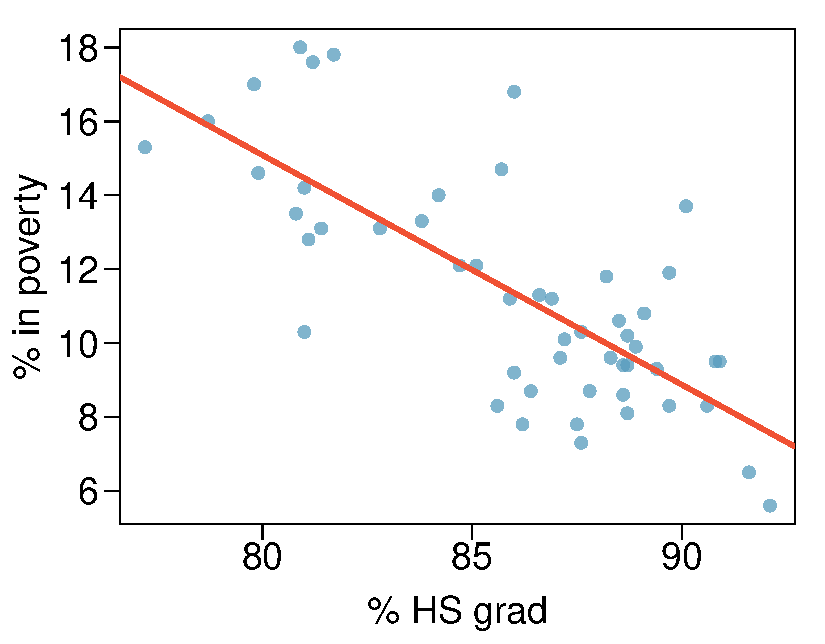
\includegraphics[width=\textwidth]{plots/poverty_hsgrad_line.pdf}
\end{figure}
\end{column}
\end{columns}
\vfill

\pause What does 64.68 represent here? \pause Poverty rate for states with no high-school grads. Not sensible/interpretable.\\~\\

\pause How is 0.62 interpreted here? \pause Increasing \% of high-school grads by 1\% is associated with 0.62\% decrease in poverty rate \textit{on average}.
\end{frame}

\begin{frame}{Simple linear regression using matrices}
Note the simple linear regression model for all examples
\begin{align*}
    Y_1&=\beta_0 + \beta_1x_1+\epsilon_1,\\
    &\vdots\\
    Y_n&=\beta_0+\beta_1x_n+\epsilon_n
\end{align*}
can be written in matrix terms as
$$
\underbrace{\begin{bmatrix}
Y_1\\
\vdots\\
Y_n
\end{bmatrix}}_{\mathbf{y}}=
\underbrace{\begin{bmatrix}
1 & x_1\\
\vdots & \vdots\\
1 & x_n
\end{bmatrix}}_{\mathbf{X}}
\underbrace{\begin{bmatrix}
\beta_0\\
\beta_1
\end{bmatrix}}_{\boldsymbol\beta}
+\underbrace{\begin{bmatrix}
\epsilon_1\\
\vdots\\
\epsilon_n
\end{bmatrix}}_{\boldsymbol\epsilon},
$$
or equivalently
$$
\mathbf{y}=\mathbf{X}\boldsymbol{\beta}+\boldsymbol{\epsilon}
$$
\end{frame}

\begin{frame}{Remark on $\mathbf{X}^\top\mathbf{X}$}
Notice that
\begin{align*}
    \mathbf{X}^\top\mathbf{X}&=
    \begin{bmatrix}
    1 & \ldots & 1\\
    x_1 & \ldots & x_n
    \end{bmatrix}\begin{bmatrix}
    1 & x_1\\
    \vdots & \vdots\\
    1 & x_n
    \end{bmatrix}\\
    &=\begin{bmatrix}
    n & \sum x_i\\
    \sum x_i & \sum x_i^2
    \end{bmatrix}
\end{align*}
\end{frame}

\section{Convexity}
\begin{frame}{Convex function of one variable}
\begin{columns}
\begin{column}{.5\textwidth}
\begin{definition}
A function $f:\mathbb{R}\to\mathbb{R}$ is \textbf{convex} (\textbf{concave up}) if \pause
\begin{multline*}
f(tx_1+(1-t)x_2)\\\le tf(x_1)+(1-t)f(x_2)    
\end{multline*}
for all $x_1,x_2\in\mathrm{dom}f$ and all $t\in[0,1]$. 
\end{definition}
\end{column}
\begin{column}{.5\textwidth}
\begin{figure}
    \centering
    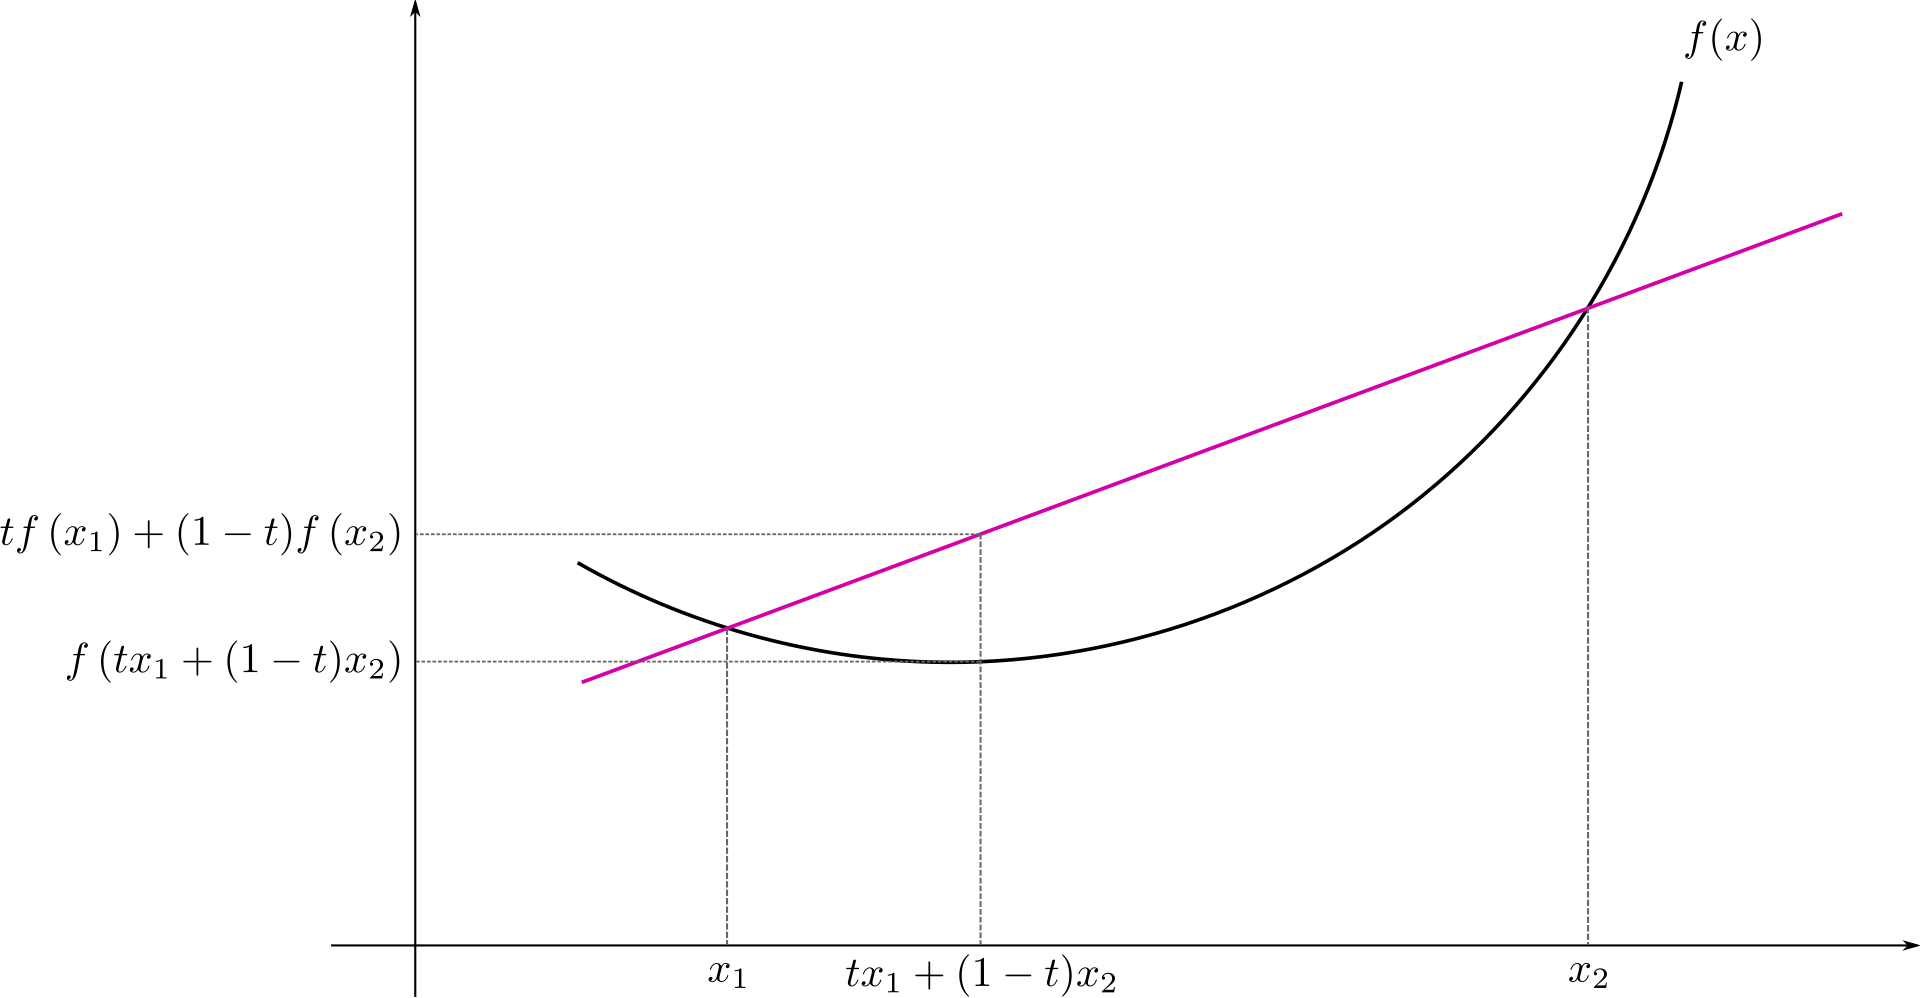
\includegraphics[width=\textwidth]{plots/conv_func.png}
\end{figure}
\end{column}
\end{columns}
\vfill

\pause How do we usually check convexity for a twice-differentiable function? \pause
\begin{theorem}
If $f''\ge0$, then $f$ is convex.
\end{theorem}
\end{frame}

\iffalse
\begin{frame}{Convex sets}
A set $\mathcal{X}\subset\mathbb{R}^d$ is \textbf{convex} if
$$
t\mathbf{x}+(1-t)\mathbf{y}\in\mathcal{X}
$$
for all $\mathbf{x},\mathbf{y}\in\mathcal{X}$ and all $t\in[0, 1]$.
\begin{figure}
    \centering
    \includegraphics[width=.9\textwidth]{plots/conv}
\end{figure}
\end{frame}
\fi

\begin{frame}{Hessian}
The \textbf{Hessian} matrix of $f:\,\mathbb{R}^d\to\mathbb{R}$ is a matrix of second-order partial derivatives:
$$
\mathbf{H}(f)=\begin{bmatrix}
\frac{\partial^2 f}{\partial x_1^2} & \cdots & \frac{\partial^2 f}{\partial x_1\partial x_d} \\
\vdots & \ddots & \vdots \\
\frac{\partial^2 f}{\partial x_d\partial x_1} & \cdots & \frac{\partial^2 f}{\partial x_d^2}
\end{bmatrix}\qquad\text{i.e.}\qquad\mathbf{H}_{ij}=\frac{\partial^2 f}{\partial x_i\partial x_j}
$$
\onslide<2->{If the partial derivatives are continuous, the order of differentiation can be interchanged, so the Hessian matrix will be symmetric.}
\end{frame}

\begin{frame}{Convex function of multiple variables}
\begin{columns}
\begin{column}{.5\textwidth}
Assume $f:\,\mathbb{R}^d\to\mathbb{R}$. A function $f$ is \textbf{convex} if \pause
\begin{multline*}
f(t\mathbf{x}+(1-t)\mathbf{y})\\\le tf(\mathbf{x})+(1-t)f(\mathbf{y})
\end{multline*}
for all $\mathbf{x}, \mathbf{y}\in\mathrm{dom}f$ and all $t\in[0,1]$.    
\end{column}
\begin{column}{.5\textwidth}
\begin{figure}
    \centering
    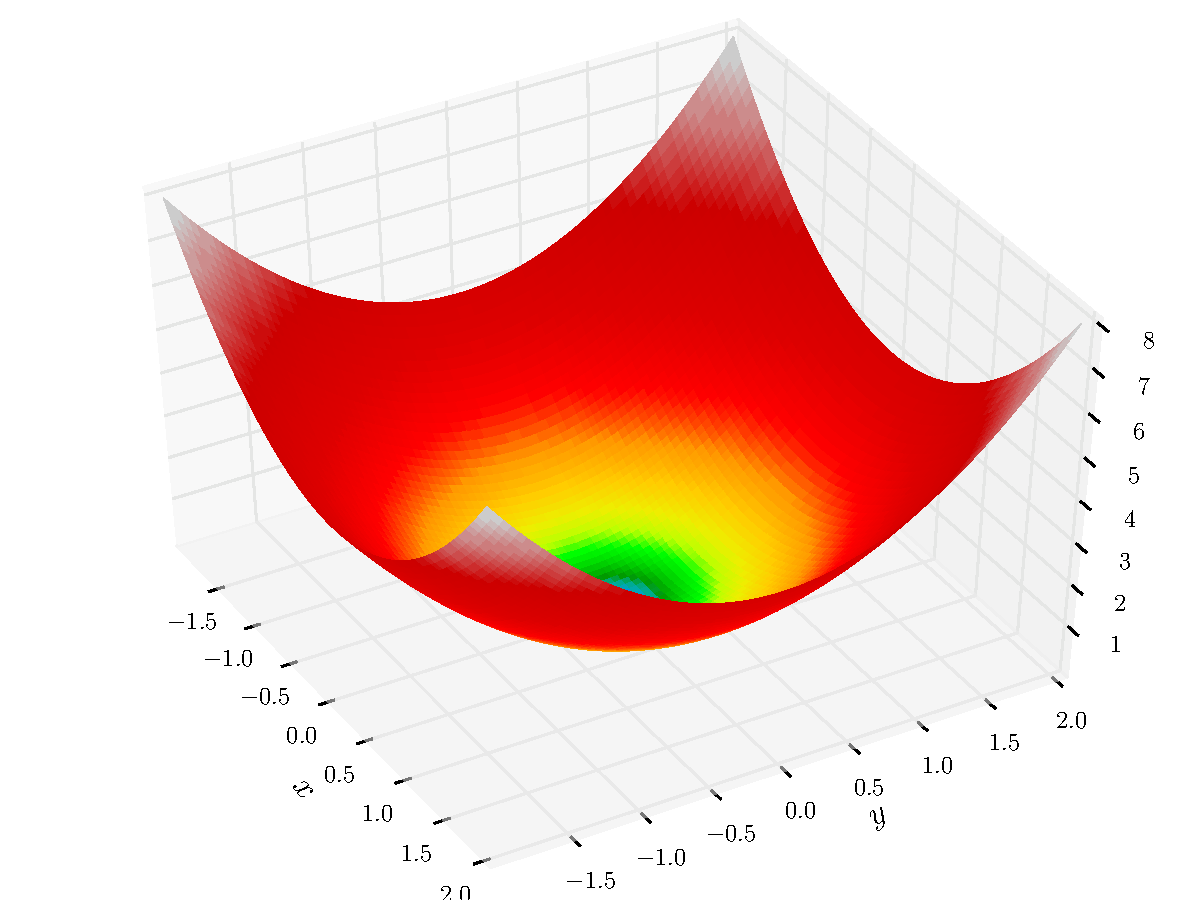
\includegraphics[width=\textwidth]{plots/Sphere_function_in_3D.pdf}
\end{figure}
\end{column}
\end{columns}
\vfill

\pause
\begin{theorem}
If $\mathbf{H}\succeq\mathbf{0}$, then $f$ is convex.
\end{theorem}
\vfill

\pause $\mathbf{H}\succeq\mathbf{0}$ denotes that $\mathbf{H}$ is a \textbf{positive semi-definite} matrix. What does this mean? \pause $\mathbf{a}^\top\mathbf{Ha}\ge0$ for any $\mathbf{a}\in\mathbb{R}^d$.

\end{frame}


\begin{frame}{Why are we interested in convex functions?}
    \pause {Convex functions do not have saddle points or local minima.\\~\\}
    
    \pause {\begin{theorem}
    If $f$ is convex, then any local minimum of $f$ is also a \textit{global} minimum.\\~\\
    \end{theorem}}
    
    \pause {$\Rightarrow$ We can find any stationary point and guarantee that it is the global minimum.\\~\\
    }
    
    \pause What is a stationary point? A point $\mathbf{x}_0$ is called \textbf{stationary} if $\nabla f(\mathbf{x}_0)=0$.
\end{frame}

\section{Parameter Estimation}

\subsection{Least Squares Estimation (LSE)}
\begin{frame}{Eyeballing the line}
\begin{columns}
\begin{column}{.5\textwidth}
Which of the following appears to be the line that best fits the linear relationship between \% in poverty and \% HS grad?\\~\\

\onslide<2->{(a)}
\end{column}
\begin{column}{.5\textwidth}
\begin{figure}
    \centering
    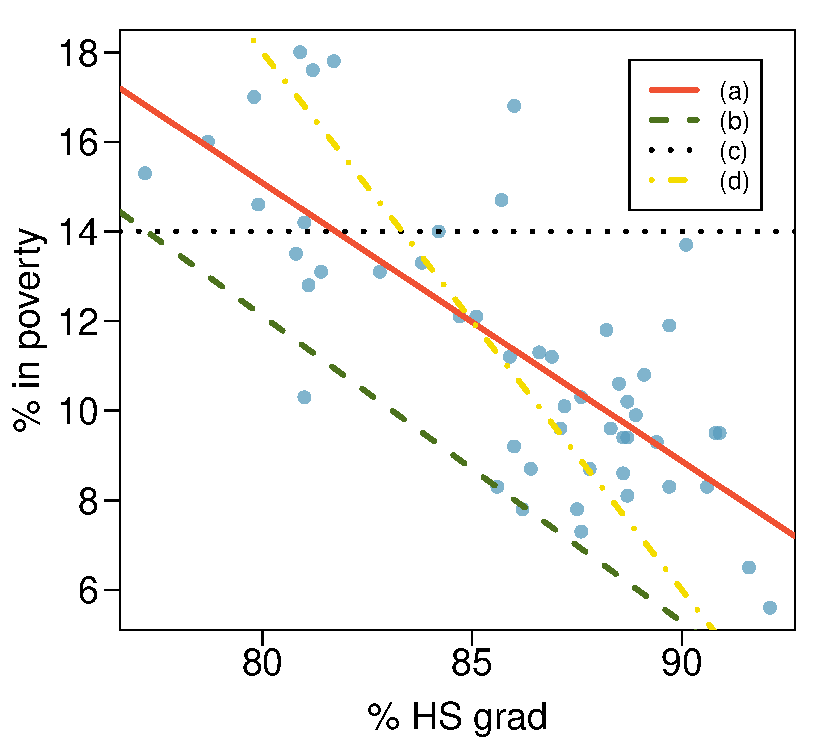
\includegraphics[width=\textwidth]{plots/poverty_hsgrad_manylines.pdf}
\end{figure}
\end{column}
\end{columns}
\end{frame}

\begin{frame}{Residuals}
\textbf{Errors} are simply $\epsilon_i=Y_i-(\beta_0+\beta_1x_i)$,\\
\pause\textbf{Residuals} are \textit{estimated} errors: $e_i=Y_i-(b_0+b_1 x_i)$ once $\beta_0$ and $\beta_1$ have been replaced by their estimates $b_0$ and $b_1$.
\begin{columns}
\begin{column}{.5\textwidth}
\begin{figure}
    \centering
    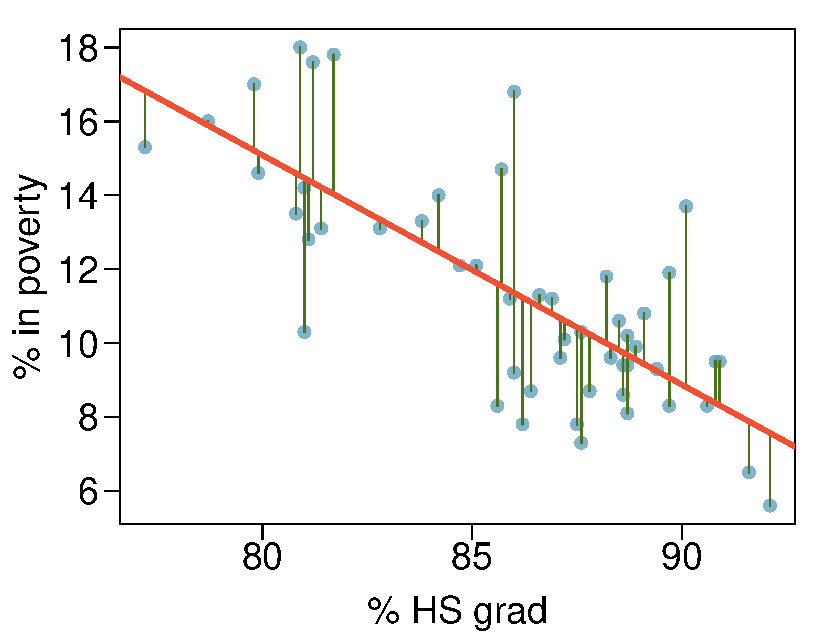
\includegraphics[width=\textwidth]{plots/poverty_hsgrad_res.pdf}
\end{figure}
\end{column}
\begin{column}{.5\textwidth}
\pause We want a line that has smallest possible residuals:
$$
\min_{b_0,b_1}\sum_{i=1}^n e_i^2
$$
\pause This is called \textbf{least squares estimation (LSE)}. 
\end{column}
\end{columns}
\pause Why don't we minimize the sum $\sum_{i=1}^n e_i$ instead? \pause Positive and negative residuals will compensate each other $\Rightarrow$ we won't be sure that the magnitudes $|e_i|$ are small.
\end{frame}

\begin{frame}{Least squares estimation of $\beta_0$ and $\beta_1$}
\begin{theorem}
The function $Q(\beta_0, \beta_1)=\sum_{i=1}^n[Y_i-(\beta_0+\beta_1 x_i)]^2$ has the global minimum at
\begin{align*}
b_1:=\hat\beta_1&=\frac{\sum_{i=1}^n(x_i-\bar{x})(Y_i-\bar{Y})}{\sum_{i=1}^n(x_i-\bar{x})^2}\\
b_0:=\hat\beta_0&=\bar{Y}-\hat\beta_1\bar{x}
\end{align*}
\end{theorem}
\pause\structure{Proof.} First derivatives of $Q$:
$$
\frac{\partial Q}{\partial\beta_1}=\sum_{i=1}^n2(Y_i-\beta_0-\beta_1x_i)(-x_i)=-2\left[\sum_{i=1}^n x_i Y_i-\beta_0\sum_{i=1}^n x_i - \beta_1\sum_{i=1}^n x_i^2\right],
$$
\pause $$
\frac{\partial Q}{\partial\beta_0}=\sum_{i=1}^n 2(Y_i-\beta_0-\beta_1 x_i)(-1)=-2\left[\sum_{i=1}^n Y_i-n\beta_0-\beta_1\sum_{i=1}^n x_i\right].
$$
\end{frame}

\begin{frame}{Two equations in two unknowns}
Setting these equal to zero, we have
\begin{align}
\sum x_i Y_i&=\beta_0\sum x_i+\beta_1\sum x_i^2\label{eq:first}\\
\sum Y_i&=n\beta_0+\beta_1\sum x_i\label{eq:second}
\end{align}
\pause Multiply \eqref{eq:first} by $n$ and multiply \eqref{eq:second} by $\sum x_i$ and subtract yielding
$$
n\sum x_i Y_i-\sum x_i\sum Y_i = \beta_1\left[n\sum x_i^2-\left(\sum x_i\right)^2\right].
$$
\pause Solving for $\beta_1$ we get
$$
\hat\beta_1=\frac{n\sum x_i Y_i-\sum x_i\sum Y_i}{n\sum x_i^2-\left(\sum x_i\right)^2}=\frac{\sum x_i Y_i - n\bar{Y}\bar{x}}{\sum x_i^2-n\bar{x}^2}.
$$
Plugging this into \eqref{eq:second}, we have $\hat\beta_0=\bar{Y}-\hat\beta_1\bar{x}$.
\end{frame}

\begin{frame}{Convexity of $Q$}
How can we show that $Q(\beta_0,\beta_1)$ is convex? \pause Its Hessian should be positive semi-definite.\\~\\

\pause Second-order partial derivatives of $Q$:
$$
\frac{\partial^2 Q}{\partial\beta_0^2}=2n,\quad\frac{\partial^2 Q}{\partial\beta_1^2}=2\sum x_i^2,\quad
\frac{\partial^2 Q}{\partial\beta_1\partial\beta_0}=2\sum x_i
$$
\pause Hessian of $Q$:
$$
\mathbf{H}=2\cdot\begin{bmatrix}
n & \sum x_i \\
\sum x_i & \sum x_i^2
\end{bmatrix}=2\mathbf{X}^\top\mathbf{X}
$$
\pause For an arbitrary $\mathbf{a}=(a_1, a_2)$ we have
\begin{align*}
\mathbf{a}^\top\mathbf{H}\mathbf{a}&=\begin{bmatrix}
a_1 & a_2
\end{bmatrix}\cdot2\cdot\begin{bmatrix}
n & \sum x_i \\
\sum x_i & \sum x_i^2
\end{bmatrix}\begin{bmatrix}
a_1 \\ a_2
\end{bmatrix}=\mathbf{a}^\top 2\mathbf{X}^\top\mathbf{X}\mathbf{a}\\
&=2(\mathbf{X}\mathbf{a})^\top(\mathbf{X}\mathbf{a})=2\|\mathbf{X}\mathbf{a}\|^2\ge0\quad\Rightarrow\quad \mathbf{H}\succeq\mathbf{0}
\end{align*}
\end{frame}

\subsection{Maximum Likelihood Estimation (MLE)}
\begin{frame}{Probabilistic Setup}
    Assume
    $$
    Y_i=\beta_0+\beta_1 x_i+\epsilon_i,\qquad\pause\epsilon_i\,\,{\stackrel{\text{iid}}{\sim}}\,\,\mathcal{N}(0,\sigma^2)
    $$%
    \onslide<3->{This is equivalent to
    $$
    Y_i\,{\stackrel{\text{ind}}{\sim}}\,\mathcal{N}(\beta_0+\beta_1 x_i,\sigma^2)\qquad(\text{Why?})
    $$}%
    \onslide<4->{This means that p.d.f. of $Y_i$ is
    $$
    f_{Y_i}({y})=\frac{1}{\sqrt{2\pi \sigma^2}}\exp\left(-\frac{[y-(\beta_0+\beta_1 x_i)]^2}{2\sigma^2}\right) 
    $$
    }
\end{frame}

\begin{frame}{Properties of the residuals}
\begin{columns}
\begin{column}{.5\textwidth}
\begin{figure}
    \centering
    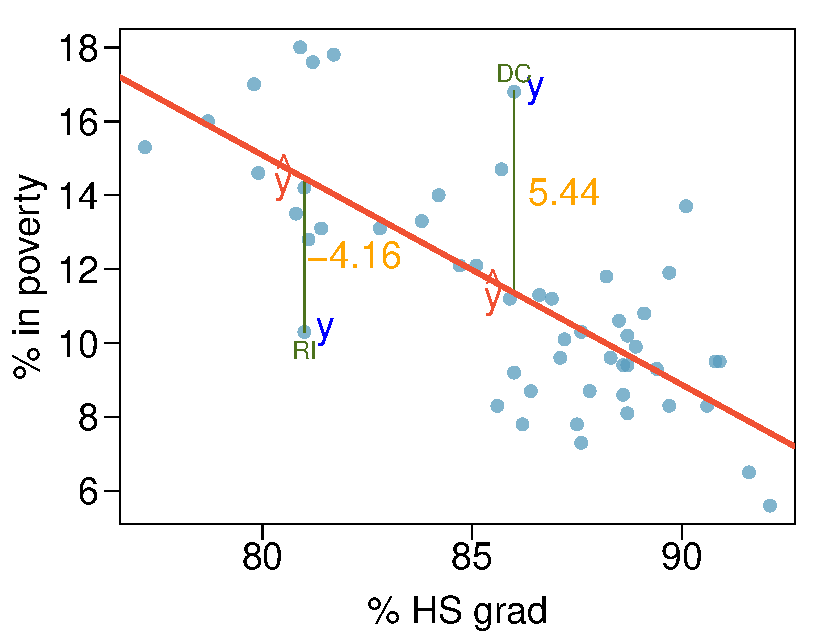
\includegraphics[width=\textwidth]{plots/poverty_hsgrad_res_text.pdf}
\end{figure}
\end{column}
\begin{column}{.5\textwidth}
Denote $\hat{Y}_i=\hat{\beta}_0+\hat{\beta}_1 x_i$.\\~\\
\pause Residuals are differences between observed and predicted responses:
$$
e_i=Y_i-\hat{Y}_i
$$
\end{column}
\end{columns}
\vfill

\begin{exe} Show that
\begin{itemize}
\item \pause $\sum_{i=1}^n e_i=0$ \pause(follows from \eqref{eq:second}),
\item \pause $\sum_{i=1}^n x_i e_i = 0$ (follows from \eqref{eq:first})
\item \pause $\sum_{i=1}^n \hat{Y}_i e_i = 0$ (from the previous two),
\item \pause Least squares line always goes through $(\bar{x}, \bar{Y})$.
\end{itemize}
\end{exe}
\end{frame}

\begin{frame}{Maximum Likelihood Estimation (MLE)}
    The \textit{likelihood function} for the sample $Y_1,\ldots,Y_n$ given parameters $\beta_0$, $\beta_1$, $\sigma$ is
    $$
    \mathcal{L}(\beta_0, \beta_1,\sigma^2)=\prod_i f_{Y_i}({Y}_i)=\prod_i\frac{1}{\sqrt{2\pi \sigma^2}}\exp\left(-\frac{[Y_i-(\beta_0+\beta_1 x_i)]^2}{2\sigma^2}\right)
    $$
    \onslide<2->{\begin{exe} Find the MLE for $\beta_0$ and $\beta_1$:
    $$
    (\hat{\beta}_{0,\text{MLE}},\hat{\beta}_{1,\text{MLE}})=\argmax_{\beta_0, \beta_1}\mathcal{L}(\beta_0,\beta_1,\sigma^2)
    $$%
    \onslide<3->{Show that
    $$
    \max_{\beta_0,\beta_1}\mathcal{L}(\beta_0,\beta_1,\sigma^2)\qquad\Leftrightarrow\qquad\min_{\beta_0,\beta_1}Q(\beta_0,\beta_1)
    $$}\end{exe}}%
    \onslide<4->{$\Rightarrow$ MLE is a probabilistic justification for the LSE.}
\end{frame}

\iffalse
\begin{frame}{Properties of least squares estimators}
The line $\hat{Y}=b_0+b_1x$ is called the \textit{least squares} estimated regression line. Why are the least squares estimates $(b_0, b_1)$ ``good''?
\begin{itemize}
\item They are unbiased: $\E[b_0]=\beta_0$ and $\E[b_1]=\beta_1$.
\item Among all linear unbiased estimators, they have the smallest variance. They are \textbf{b}est \textbf{l}inear \textbf{u}nbiased \textbf{e}stimators, BLUEs.
\end{itemize}
We will show the first property next. The second property is formally called ``Gauss-Markov'' theorem (1.11) and is proved in linear models (p. 18).
\end{frame}

\begin{frame}{2.1 and 2.2: Unbiasedness}
\textbf{$b_0$ and $b_1$ are unbiased} (Section 2.1, p.42) Recall that least-squares estimators $(b_0, b_1)$ are given by:
$$
b_1=\frac{n\sum x_i Y_i-\sum x_i\sum Y_i}{n\sum x_i^2-\left(\sum x_i\right)^2}=\frac{\sum x_i Y_i-n\bar{Y}\bar{x}}{\sum x_i^2-n\bar{x}^2},
$$
and
$$
b_0=\bar{Y}-b_1\bar{x}.
$$
Note that the numerator of $b_1$ can be written
$$
\sum x_i Y_i - n\bar{Y}\bar{x}=\sum x_i Y_i-\bar{x}\sum Y_i = \sum(x_i-\bar{x})Y_i
$$
\end{frame}

\begin{frame}{Keep going...}
Then the expectation of $b_1$'s numerator is
\begin{align*}
\E\left[\sum(x_i-\bar{x})Y_i\right]&=\sum(x_i-\bar{x})\E[Y_i]\\
&=\sum(x_i-\bar{x})(\beta_0+\beta_1 x_i)\\
&=\beta_0\sum x_i-n\bar{x}\beta_0+\beta_1\sum x_i^2-n\bar{x}^2\beta_1\\
&=\beta_1\left(\sum x_i^2-n\bar{x}^2\right)
\end{align*}
Finally,
\begin{align*}
\E[b_1]&=\frac{\E\left[\sum(x_i-\bar{x})Y_i\right]}{\sum x_i^2-n\bar{x}^2}\\
&=\frac{\beta_1\left(\sum x_i^2-n\bar{x}^2\right)}{\sum x_i^2-n\bar{x}^2}\\
&=\beta_1.
\end{align*}
\end{frame}

\begin{frame}{$\E[b_0]=\beta_0$}
Also,
\begin{align*}
\E[b_0]&=\E(\bar{Y}-b_1\bar{x})\\
&=\frac1n\sum\E[Y_i]-\E[b_1]\bar{x}\\
&=\frac1n\sum(\beta_0+\beta_1 x_i)-\beta_1\bar{x}\\
&=\frac1n(n\beta_0+n\beta_1\bar{x})-\beta_1\bar{x}\\
&=\beta_0.
\end{align*}
As promised, $b_1$ is unbiased for $\beta_1$ and $b_0$ is unbiased for $\beta_0$.
\end{frame}

\begin{frame}[fragile]
\frametitle{Whale Selenium, SAS code}
\begin{itemize}
\item \texttt{proc reg} and \texttt{proc glm} fit regression models.
\item Both include a \texttt{model} statement that tells SAS what the explanatory variable(s) are (on the right of = separated by spaces) and the response (on the left).
\begin{scriptsize}
\begin{verbatim}
data whale;
input liver tooth @@;
label liver="Liver Se (mcg/g)"; label tooth="Tooth Se (ng/g)";
datalines;
 6.23 140.16  6.79 133.32  7.92 135.34  8.02 127.82  9.34 108.67
10.00 146.22 10.57 131.18 11.04 145.51 12.36 163.24 14.53 136.55
15.28 112.63 18.68 245.07 22.08 140.48 27.55 177.93 32.83 160.73
36.04 227.60 37.74 177.69 40.00 174.23 41.23 206.30 45.47 141.31
;
proc reg;
  model liver=tooth;
\end{verbatim}
\end{scriptsize}
\end{itemize}
\end{frame}

\begin{frame}{Whale Selenium, SAS output}
\begin{center}
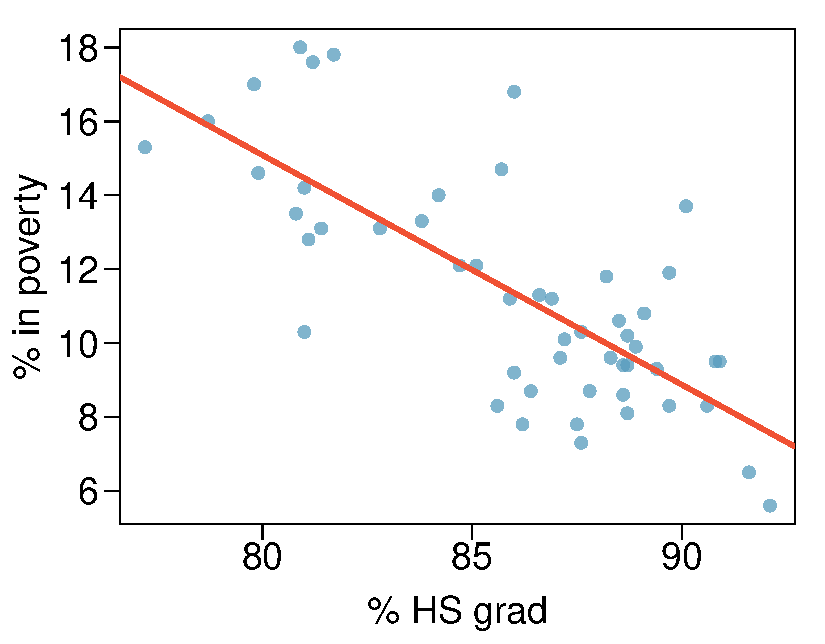
\includegraphics[scale=0.3]{plots/poverty_hsgrad_line.pdf}
\end{center}
From this $b_0=-10.69$, $b_1=0.2004$, and $\hat{\sigma}=11.65$.\\
Interpretation of each?
\end{frame}

\begin{frame}{Toluca data (p. 19)}
\begin{itemize}
\item Toluca makes replacement parts for refrigerators.
\item We consider one particular part, manufactured in varying lot sizes.
\item Takes time to set up production regardless of lot size; this time plus machining \& assembly makes up work hours.
\item Want to relate work hours to lot size.
\item $n=25$ pairs $(x_i, Y_i)$ were obtained.
\end{itemize}
\end{frame}

\begin{frame}[fragile]
{Toluca data, scatterplot \& regression in SAS}
\begin{verbatim}
data toluca;
input size hours @@;
label size="Lot Size (parts/lot)"; label hours="Work Hours";
datalines;
 80 399  30 121 50 221 90 376 70 361  60 224 120 546
 80 352 100 353 50 157 40 160 70 252  90 389  20 113
110 435 100 420 30 212 50 268 90 377 110 421  30 273
 90 468  40 244 80 342 70 323
;
proc sgscatter; plot hours*size; run;
options nocenter;
proc reg; model hours=size; run;
\end{verbatim}
\end{frame}

\begin{frame}{Toluca data, SAS output}
\begin{center}
\includegraphics[scale=0.4]{plots/Toluca-out}
\end{center}
\end{frame}

\begin{frame}{Toluca data}
\begin{center}
\includegraphics[scale=0.4]{plots/Toluca-out2}
\end{center}
\end{frame}

\begin{frame}{Toluca}
The fitted model is
$$
\reallywidehat{\rm hours} = 62.37 + 3.570 \text{ lot size}
$$
\begin{itemize}
\item A lot size of $x=65$ takes $\hat{Y}=62.37+3.570(65)=294$ hours to finish, \textit{on average}
\item For each unit increase in lot size, the mean time to finish increases by 3.57 hours.
\item Increasing the lot size by 10 parts increases the time by 35.7 hours, about a week.
$b_0=62.37$ is only interpretable for lots of size zero. What does that mean here?
\end{itemize}
\end{frame}

\begin{frame}{1.6 Residuals \& fitted values}
\begin{itemize}
\item The $i$th \alert{fitted value} is $\hat{Y}=b_0+b_1 x_i$.
\item The points $(x_1, \hat{Y_1})$, \ldots, $(x_n, \hat{Y}_n)$ fall on the line $y=b_0+b_1 x$, the points $(x_1, Y_1)$, \ldots, $(x_n, Y_n)$ do not.
\item The $i$th \alert{residual} is
$$
e_i=Y_i-\hat{Y}_i=Y_i-(b_0+b_1 x_i),\qquad i=1,\ldots,n,
$$
the difference between observed and fitted values.
\item $e_i$ estimates $\epsilon_i$.
\end{itemize}
\end{frame}
\fi



\begin{frame}{Estimating $\sigma^2$}
Recall that $\sigma^2=\Var[\epsilon_i]$.\\~\\

\pause A natural estimator of $\sigma^2$ is \pause $
\hat{\sigma}^2=\frac1n\sum_{i=1}^n (e_i-\bar{e})^2=\frac1n\sum_{i=1}^n e_i^2$ \pause (why $\bar{e}=0$? \pause because $\sum e_i=0$)\\~\\

\pause In Chapter 5, we will show that $\frac{\sum e_i^2}{\sigma^2}\sim\chi^2_{n-2}$. This implies $\E[\hat{\sigma}^2]=\frac{n-2}{n}\sigma^2$.
\pause I.e., $\hat{\sigma}^2$ is a biased estimator of $\sigma^2$, and we prefer the unbiased version:
$$
\frac{n}{n-2}\hat{\sigma}^2=\frac1{n-2}\sum_{i=1}^n e_i^2=\frac{1}{n-2}\sum_{i=1}^n(Y_i-b_0-b_1 x_i)^2:=\mathrm{MSE}.
$$
which is referred to as \textbf{mean squared error} (\textbf{MSE}).
\end{frame}

\begin{frame}[fragile]
\frametitle{Parameter estimation in \texttt{R}: Poverty vs HS grad rate}
{\color{blue} \url{https://raw.githubusercontent.com/zh3nis/MATH440/main/chp01/poverty.R}}
\begin{columns}
\begin{column}{.5\textwidth}
\begin{small}
\begin{verbatim}
Coefficients:
            Estimate     
(Intercept) 64.78097 
Graduates   -0.62122 

Residual standard error: 2.082
\end{verbatim}    
\end{small}
\end{column}
\begin{column}{.5\textwidth}
\begin{figure}
    \centering
    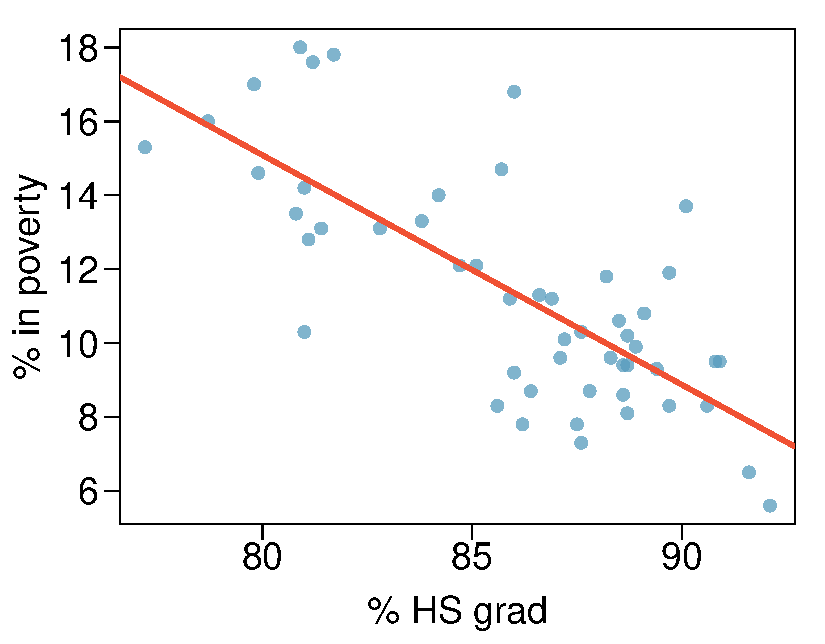
\includegraphics[width=\textwidth]{plots/poverty_hsgrad_line.pdf}
\end{figure}
\end{column}
\end{columns}

\vfill
\pause 
The regression line is $y=\underbrace{64.78}_{b_0}-\underbrace{0.62}_{b_1}x$.\\~\\
$\sqrt{\mathrm{MSE}}=2.08$ is an estimate of $\sigma$.
\end{frame}

\end{document}